\documentclass[bachelor, och, labwork]{shiza}

\usepackage{subfigure}
\usepackage{tikz,pgfplots}
\pgfplotsset{compat=1.5}
\usepackage{float}

\usepackage{titlesec}
\setcounter{secnumdepth}{4}
\titleformat{\paragraph}
{\normalfont\normalsize}{\theparagraph}{1em}{}
\titlespacing*{\paragraph}
{35.5pt}{3.25ex plus 1ex minus .2ex}{1.5ex plus .2ex}

\titleformat{\paragraph}[block]
{\hspace{1.25cm}\normalfont}
{\theparagraph}{1ex}{}
\titlespacing{\paragraph}
{0cm}{2ex plus 1ex minus .2ex}{.4ex plus.2ex}

% --------------------------------------------------------------------------%


\usepackage[T2A]{fontenc}
\usepackage[utf8]{inputenc}
\usepackage{graphicx}
\graphicspath{ {./images/} }
\usepackage{tempora}

\usepackage[sort,compress]{cite}
\usepackage{amsmath}
\usepackage{amssymb}
\usepackage{amsthm}
\usepackage{fancyvrb}
\usepackage{listings}
\usepackage{listingsutf8}
\usepackage{longtable}
\usepackage{array}
\usepackage[english,russian]{babel}

\usepackage[colorlinks=true]{hyperref}
\usepackage{url}

\usepackage{underscore}
\usepackage{setspace}
\usepackage{indentfirst} 
\usepackage{mathtools}
\usepackage{amsfonts}
\usepackage{enumitem}
\usepackage{tikz}
\usepackage{minted}

\newcommand{\eqdef}{\stackrel {\rm def}{=}}
\newcommand{\specialcell}[2][c]{%
\begin{tabular}[#1]{@{}c@{}}#2\end{tabular}}

\renewcommand\theFancyVerbLine{\small\arabic{FancyVerbLine}}


\begin{document}

% \chair{Кафедра теоретических основ компьютерной безопасности и криптографии}

\title{Классификация бинарных отношений и системы замыканий}

\course{3}

\group{331}

\department{факультета КНиИТ}

\napravlenie{10.05.01 "--- Компьютерная безопасность}

\author{Никитина Арсения Владимировича}

\satitle{ассистент}

\saname{Р. А. Фарахутдинов}

\date{2021}

\maketitle

%-------------------------------------------------------------------------------

\tableofcontents

\intro

Существует определенная классификация бинарных отношений в зависимости от их 
свойств. Задачей данной работы является рассмотрение основных свойств бинарных 
отношений, а также их классификация. В зависимости от класса бинарного 
отношения, на нем можно определить замыкание: относительно рефлексивности,
симметричности и транзитивности. Для этого требуется понимать, каким образом 
происходит классификация отношений в зависимости от множеств, которыми они могут
задаваться.

\section{\textbf{Цель работы и порядок ее выполнения}}

\textbf{Цель работы} "--- изучение основных свойств бинарных отношений и 
операций замыкания бинарных отношений.

Порядок выполнения работы:

\begin{enumerate}

    \item Разобрать основные определения видов бинарных отношений и разработать
    алгоритм классификации бинарных отношений.

    \item Изучить свойства бинарных отношений и рассмотреть основные системы
    замыкания на множестве бинарных отношений.

    \item Разработать алгоритмы построения основных замыканий бинарных отношений.

\end{enumerate}

\section{Теоретические сведения}

\subsection{Основные определения видов бинарных отношений и их алгоритмы}

\subsubsection{Определение бинарного отношения}

Подмножества декартова произведения $A \times B$ множеств $A$ и $B$ называются
\textbf{бинарными отношениями} между элементами множеств $A$ и $B$ и 
обозначаются строчными греческими буквами $\rho$, $\rho_1$ и т.п.

Для бинарного отношения $\rho\subset A \times B$ область определения $D_\rho$ и 
множество значений $E_\rho$ определяется как подмножества соответствущих множеств 
$A ~\text{и}~ B$ по следующим формулам:

\begin{center}
    $D_\rho ~ = ~ \{a : (a, b) \in\rho ~ \text{для некоторого} ~ b \in B\}$,
    $E_\rho ~ = ~ \{b : (a, b) \in\rho ~ \text{для некоторого} ~ a \in A\}$.
\end{center}

\subsubsection{Основные свойства бинарных и алгоритмы их определения}

Бинарное отношение $\rho \subset A \times A$ называется:

\begin{enumerate}
    
    \item \textit{рефлексивным}, если $(a,a)\in\rho~\forall a \in A$.
    
    \item \textit{антирефлексивным}, если $(a,a)\not\in\rho~\forall a \in A$.
    
    \item \textit{симметричным}, если $(a,b)\in\rho\Rightarrow (b,a)\in\rho~\forall a,b\in A$.
    
    \item \textit{антисимметричным}, если $(a,b) \in\rho~\text{и}~(b,a) \in\rho ~ \Rightarrow a = b ~\forall a,b \in A$.
    
    \item \textit{транзитивным}, если $(a,b)\in\rho ~\text{и}~ (b,c)\in\rho\Rightarrow (a,c) \in\rho ~\forall a,b,c \in A $.

\end{enumerate}

Далее представлена программная реализация определения свойств бинарных 
отношений.

Итак, чтобы задать матрицу $M(\rho)_{ij}=a_{ij}$ бинарного отношения $\rho$ размерности
$N \times N$, необходимо:

\begin{enumerate}

    \item Определить мощность бинарного отношения, то есть количество
    элементов в строках и столбцах матрицы.

    \item Если упорядоченная пара $(a, b)$ присутствует в отношении, то 
    $M_{i-1,j-1} = 1$, иначе $M_{i-1,j-1} = 0$.

\end{enumerate}

Выполним проверку свойств \textbf{рефлексивности} и \textbf{антирефлексивности}:

\textit{Вход.} Матрица $M(\rho)_{ij}$ бинарного отношения $\rho$ размерности
$N \times N$

\textit{Выход.} Пара логических значений \textit{Истина} или \textit{Ложь}.

\begin{enumerate}
    
    \item Завести логические переменные для рефлексивности и антирефлексивности и присвоить
    им значение \textit{Истина}.
    
    \item Циклически проверить (для $i ~\text{от}~ 0 ~\text{до}~ n-1$), какие 
    числа стоят на главной диагонали матрицы ($M_{ii}$).

    \item Если $M_{ii} = 1$, то присвоить переменной для антирефлексивности значение
    \textit{Ложь}, если же $M_{ii} = 0$, то присвоить значение \textit{Ложь} переменной для
    рефлексивности.

    \item Если значения обеих логических переменных стали равны \textit{Ложь}, то
    ответ - пара \textit{Ложь, Ложь}.
    
    \item Если цикл завершился, то ответ - пара логических переменных.

\end{enumerate}


Выполним проверку свойства свойства \textbf{симметричности и антисимметричности}:

Свойство симметричности выполняется для отношения, заданного матрицей, если
элементы, симметричные относительно главной диагонали равны.

\textit{Вход.} Матрица $M(\rho)_{ij}$ бинарного отношения $\rho$ размерности
$N \times N$

\textit{Выход.} Пара логических значений \textit{Истина} или \textit{Ложь}.

\begin{enumerate}
    
    \item Завести логические переменные для симметричности и антисимметричности 
    и присвоить им значение \textit{Истина}.

    \item Циклически проверить (для $i ~\text{от}~ 0 ~\text{до}~ n$, 
    для $j ~\text{от}~ 0 ~\text{до}~ n$), какие числа стоят на местах $M_{ij},M_{ji}$

    \item Если $M_{ij} = M_{jj}$, то присвоить значение переменной для
    антисимметричности \textit{Ложь}.
    
    \item Если значения обеих логических переменных стали равны \textit{Ложь}, то
    ответ - пара \textit{Ложь, Ложь}.
    
    \item Если цикл завершился, то ответ - пара логических переменных.

\end{enumerate}

Выполним проверку свойства свойства \textbf{транзитивности}:

Свойство транзитивности выполняется для отношения, заданного матрицей, если для 
любого фиксированного элемента $M_{k,i}=1$ из матрицы отношения, и для любого
элемента из матрицы отношения $M_{i,j}=1$, то выполняется $M_{k,j}=1$.

\textit{Вход.} Матрица $M(\rho)_{ij}$ бинарного отношения $\rho$ размерности
$N \times N$

\textit{Выход.} Логическое значение \textit{Истина или Ложь}.

\begin{enumerate}
    
    \item Завести логическую переменную транзитивности и присвоить ей значение \textit{Истина}.

    \item Циклически проверить (для $i ~\text{от}~ 0 ~\text{до}~ n$, 
    для $j ~\text{от}~ 0 ~\text{до}~ n$), какие числа стоят на местах $M_{ij},M_{ji}$
    
    \item Если $M_{k,i}=M_{i,j}=M_{k,i}=1$, то обход матрицы продолжается.
   
    \item Если же условие не выполнено, то происходит выход из цикла и алгоритм 
    определения транзитивности завершается со значением \textit{Ложь}.

    \item Если же циклический обход завершен, то алгоритм определения 
    транзитивности завершается со значением \textit{Истина}.

\end{enumerate}

\subsection{Классификация бинарных отношений}

Таким образом, в зависимости от свойств, которыми заданное бинарное отношение
обладает, его можно отнести к определенному классу: \textbf{квазипорядка,
эквивалентности} или \textbf{частичного порядка}. 

\subsubsection{Определения классов бинарных отношений}

Отношение \textit{эквивалентности} -- это такое бинарное отношение между элементами
множества $A$, для которого выполнены свойства рефлексивности, симметричности 
и транзитивности, то есть $\forall a,b,c \in A$ выполняется:
\begin{enumerate}
    \item $(a,a)\in\rho~\forall a \in A$
    \item $(a,b)\in\rho\Rightarrow (b,a)\in\rho~\forall a,b\in A$
    \item $(a,b)\in\rho ~\text{и}~ (b,c)\in\rho\Rightarrow (a,c) \in\rho ~\forall a,b,c \in A $
\end{enumerate}

Отношение \textit{квазипорядка} -- это такое бинарное отношение, между элементами
множества $A$, для которого выполнены свойства рефлексивности и транзитивности,
то есть $\forall a,b,c \in A$ выполняется:
\begin{enumerate}
    \item $(a,a)\in\rho~\forall a \in A$
    \item $(a,b)\in\rho ~\text{и}~ (b,c)\in\rho\Rightarrow (a,c) \in\rho ~\forall a,b,c \in A $
\end{enumerate}

Отношение \textit{частичного порядка} -- это такое бинарное отношение, между
элементами множества $A$, для которого выполнены свойства рефлексивности и
антисимметричности, то есть $\forall a,b,c \in A$ выполняется:
\begin{enumerate}
    \item $(a,a)\in\rho~\forall a \in A$.
    $(a,b) \in\rho~\text{и}~(b,a) \in\rho ~ \Rightarrow a = b ~\forall a,b \in A$.
\end{enumerate}


\subsubsection{Алгоритм проверки отношения на квазипорядок}

\textit{Вход.} Матрица $M(\rho)_{ij}$ бинарного отношения $\rho$ размерности
$N \times N$

\textit{Выход.} <<Отношение является отношением квазипорядка>> или <<Отношение 
не является отношением квазипорядка>>.

\begin{enumerate}

    \item Запустить проверку свойств рефлексивности и транзитивности и выполнить
    логическую операцию \& для их результатов.

    \item Если значение \textit{Истина}, то ответ <<Отношение является отношением
    квазипорядка>>.
    
    \item Если значение \textit{Ложь}, то ответ <<Отношение не является 
    отношением квазипорядка>>.

\end{enumerate}


\subsubsection{Алгоритм проверки отношения на эквивалентность}

\textit{Вход.} Матрица $M(\rho)_{ij}$ бинарного отношения $\rho$ размерности
$N \times N$

\textit{Выход.} <<Отношение является отношением эквивалентности>> или 
<<Отношение не является отношением эквивалентности>>.

\begin{enumerate}

    \item Запустить проверку свойств рефлексивности, транзитивности и симметричности
    и выполнить операцию \& для их результатов.

    \item Если получившееся значение истинно, то ответ <<Отношение является
    отношением эквивалентности>>.

    \item Если же значение ложно, то ответ <<Отношение не является отношением
    эквивалентности>>. 

\end{enumerate}


\subsubsection{Алгоритм проверки отношения на частичный порядок}

\textit{Вход.} Матрица $M(\rho)_{ij}$ бинарного отношения $\rho$ размерности
$N \times N$

\textit{Выход.} <<Отношение является
отношением частичного порядка>> или <<Отношение не является отношением 
частичного порядка>>.

\begin{enumerate}
    
    \item Запустить проверку свойств рефлексивности, транзитивности и 
    антисимметричности и выполнить операцию \& для их результатов.
    
    \item Если получившееся значение истинно, то ответ <<Отношение является
    отношением частичного порядка>>.
    
    \item Если же получившееся значение ложно, то ответ <<Отношение является
    отношением частичного порядка>>.

\end{enumerate}


\subsection{Замыкания бинарных отношений и алгоритмы их построения}

\subsubsection{Определение замыкания отношения}

\textbf{Замыканием отношения} $R$ относительно свойства $P$ называется такое
множество $R^*$, что:

\begin{enumerate}

    \item $R \subset R^*$.

    \item $R^*$ Обладает свойством $P$.

    \item $R^*$ является подмножеством любого другого отношения, содержащего $R$
    и обладающего свойством $P$. 

    То есть $R^*$ является минимальным надмножеством множества $R$, 
    выдерживается $P$.

\end{enumerate}


\subsubsection{Системы замыканий}:

Множество $Z$ подмножеств множества $A$ называется \textbf{системой замыканий}, 
если оно замкнуто относительно пересечений, т.е. выполняется: 

\begin{center}$\cap B \in Z \text{для любого подмножества} B \subset Z$.\end{center}


\textit{Лемма о системах замыканий бинарных отношений.} 
На множестве $P(A^2)$ всех бинарных отношений между элементами множества $A$ 
следующие множества являются системами замыканий:

\begin{enumerate}
    
    \item $Z_r$ - множество всех рефлексивных бинарных отношений между 
    элементами множества $A$,
    
    \item $Z_s$ – множество всех симметричных бинарных отношений между 
    элементами множества $A$,
    
    \item $Z_t$ – множество всех транзитивных бинарных отношений между 
    элементами множества $A$,
    
    \item $Z_{eq} = Eq(A)$ – множество всех отношений эквивалентности на 
    множестве $A$.
\end{enumerate}

Итак, исходя из вышесказанного, можно сделать вывод, что существуют 3 вида 
замыканий отношений: \textbf{транзитивное, симметричное, рефлексивное и
эквивалентное}.

Рассмотрим множество $A=$ \{1,2,3,4\}, на котором задано отношение 
$R=$ {(1,2),(3,4),(4,2)} 

\begin{enumerate}

    \item Замыканием $R$ относительно свойства \textbf{рефлексивности} является     
        \begin{center}

            $R^*=$ \{(1,2),(3,4),(4,2);(1,1),(2,2),(3,3),(4,4)\} 
        
        \end{center}
  
    \item Замыканием $R$ относительно свойства \textbf{симметричности} является 
        \begin{center}
    
            $R^*=$ \{(1,2),(3,4),(4,2);(2,1),(2,4),(4,3)\} 
    
        \end{center}
  
    \item Замыканием $R$ относительно свойства \textbf{транзитивности} является 
        \begin{center}
        
            $R^*=$ \{(1,2),(3,4),(4,2);(3,2)\} 
        
        \end{center}
    
    
\end{enumerate}

\subsubsection{Построение замыканий отношения}

Выполним построение замыкания отношения относительно свойства 
рефлексивности.

Для этого выполним циклический обход по всем элементам главной диагонали 
матрицы отношения $M_{ij}$ и будем проверять, находится ли элемент 
$(M_{ii},M_{ii})$ в исходном отношении.

\textit{Вход.} Матрица $M(\rho)_{ij}$ бинарного отношения $\rho$ размерности
$N \times N$

\textit{Выход.} Замыкание относительно свойства рефлексивности.

\begin{enumerate}
    \item Создать пустой список для хранения пар замыкания, а также использовать
    глобальное множество для хранения пар замыкания относительно рефлексивности.
    \item Для $i ~\text{от}~ 0 ~\text{до}~ n$.
    \item Если $M_{ii} = 0$, пару $(i + 1, i + 1)$ добавить в замыкание 
    рефлексивности и замыкание эквивалентности.    
    \item Вызвать функцию печати на экран исходного бинарного отношения.
    \item Напечатать пары замыкания.
\end{enumerate}

Выполним построение замыкания отношения относительно свойства 
симметричности.

Для этого выполним циклический обход по всем элементам матрицы 
отношения $M_{ij}$ и будем проверять, равны ли между собой элементы 
$M_{ij},M_{ji}$ в исходном отношении.

\textit{Вход.} Матрица $M(\rho)_{ij}$ бинарного отношения $\rho$ размерности
$N \times N$

\textit{Выход.} Замыкание относительно свойства симметричности.

\begin{enumerate}
    \item Создать пустой список для хранения пар замыкания, а также использовать
    глобальное множество для хранения пар замыкания относительно эквивалентности.
    \item Для $i ~\text{от}~ 0 ~\text{до}~ n$, для $j ~\text{от}~ 0 ~\text{до}~ n$.
    \item Если $M_{ij} = 1 ~\text{и}~ M_{ji} = 0$, добавить пару $(j + 1, i + 1)$
     в замыкание симметричности и замыкание эквивалентности.
    \item Вызвать функцию печати на экран исходного бинарного отношения.
    \item Напечатать пары замыкания.
\end{enumerate}

Выполним построение замыкания отношения относительно свойства транзитивности.

Выполним циклический обход по всем элементам матрицы $M_{ij}$ со всеми
фиксированными элементами $M_{ki}=1$:

\begin{enumerate}
    \item Создать пустой список для хранения пар замыкания, а также использовать
    глобальное множество для хранения пар замыкания относительно эквивалентности.
    \item Для $k ~\text{от}~ 0 ~\text{до}~ n$, для $i ~\text{от}~ 0 ~\text{до}~ n$,
    для $j ~\text{от}~ 0 ~\text{до}~ n$.
    \item Если $M_{ki}=M_{i,j}=1 ~\text{и}~ M_{ki}=0$, то добавить пару
    $(k + 1, k + 1)$ в замыкание транзитивности и замыкание эквивалентности.
    \item Вызвать функцию печати на экран исходного бинарного отношения.
    \item Напечатать пары замыкания.
\end{enumerate}


Выполним построение замыкания отношения относительно эквивалентности.

\begin{enumerate}
    \item По очереди вызвать алгоритмы построения замыканий относительно рефлексивности,
    симметричности и транзитивности.
    \item Вызвать функцию печати на экран исходного бинарного отношения.
    \item Напечатать пары замыкания, которые находятся в глобальной переменной.
\end{enumerate}


\section{Программная реализация рассмотренных алгоритмов}
    
    \subsection{Результаты тестирования программы}

        \begin{figure}[H]
            \centering
            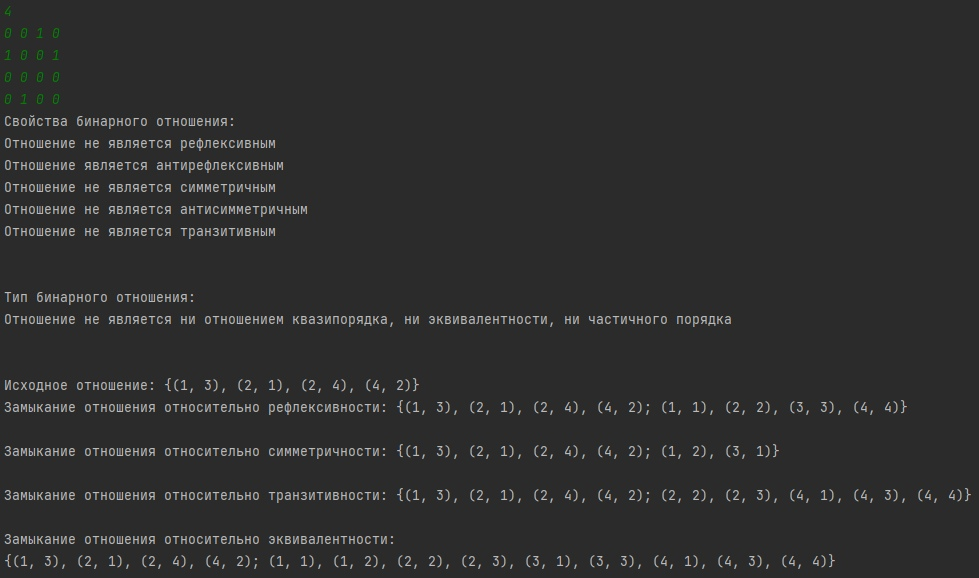
\includegraphics[width=0.8\textwidth]{pic/1.jpg}
            \caption{}
        \end{figure}
    
    \subsection{Код программы, реализующей рассмотренные алгоритмы}
    
        \inputminted[linenos,breaklines=true, fontsize=\small, style=bw]{python}{code/lab1.py}

    
    \subsection{Оценка сложности реализованных алгоритмов в программе}
    

    \subsubsection{Алгоритм проверки рефлексивности и антирефлексивности}

    Как было сказано в теоретической части лабораторной работы, для проверки 
    отношения на рефлексивность, требуется один проход по главной диагонали
    матрицы отношения, для чего требуется $O(N)$ операций.

    \subsubsection{Алгоритмы проверки рефлексивности и антирефлексивности}

    Как было сказано в теоретической части лабораторной работы, для проверки 
    отношения на свойства рефлексивности и антирефлексивности,требуется один 
    проход по главной диагонали матрицы отношения, для чего требуется $O(N)$ 
    операций.

    \subsubsection{Алгоритмы проверки симметричности и антисимметричности}
    Для проверки отношения на свойства симметричности и антисимметричности 
    в худшем случае требуется полный проход по всем элементам матрицы
    отношения, что составляет $O(N^2)$ операций.

    \subsubsection{Алгоритм проверки транзитивности}
    Для проверки отношения на свойство транзитивности требуется выполнить обход 
    по всем элементам матрицы отношения (для чего требуется один внешний цикл 
    и один вложенный) для всех фиксированных элементов из множества $A$.
    Поэтому асимптотическая оценка данного алгоритма равна $O(N^3)$ операций.

    \subsubsection{Алгоритм классификации}
    Время работы алгоритма классификации в худшем случае составляет 
    $O(N^3 + N^2 + 1)=O(N^3)$.
    

    \subsubsection{Алгоритм построения рефлексивного замыкания}
    Время работы алгоритма составляет $O(N)$

    \subsubsection{Алгоритм построения симметричного замыкания}
    Время работы алгоритма составляет $O(N^2)$

    \subsubsection{Алгоритм построения транзитивного замыкания}
    Время работы алгоритма составляет $O(N^3)$


\conclusion
В ходе лабораторной работы были рассмотрены основные свойства бинарных отношений:
рефлексивность, антирефлексивность, симметричность, антисимметричность и 
транзитивность. По определенным комбинациям свойств отношений, их можно 
классифицировать, как отношения квазипорядка (если отношение обладает 
свойствами транзитивности и рефлексивности), эквивалентности (если отношение 
является отношением квазипорядка, а также имеет свойство симметричности), а 
также отношения частичного порядка (если отношение является отношением 
квазипорядка и имеет свойство антисимметричности). Также были разработаны 
алгоритмы определения свойств отношений и их классификации. В ходе работы стало 
понятно, что самым ресурсоемким стал алгоритм определения транзитивности 
отношения, так как его реализация включает в себя тройной вложенный цикл.

\end{document}